% Options for packages loaded elsewhere
\PassOptionsToPackage{unicode}{hyperref}
\PassOptionsToPackage{hyphens}{url}
%
\documentclass[
]{article}
\usepackage{amsmath,amssymb}
\usepackage{iftex}
\ifPDFTeX
  \usepackage[T1]{fontenc}
  \usepackage[utf8]{inputenc}
  \usepackage{textcomp} % provide euro and other symbols
\else % if luatex or xetex
  \usepackage{unicode-math} % this also loads fontspec
  \defaultfontfeatures{Scale=MatchLowercase}
  \defaultfontfeatures[\rmfamily]{Ligatures=TeX,Scale=1}
\fi
\usepackage{lmodern}
\ifPDFTeX\else
  % xetex/luatex font selection
\fi
% Use upquote if available, for straight quotes in verbatim environments
\IfFileExists{upquote.sty}{\usepackage{upquote}}{}
\IfFileExists{microtype.sty}{% use microtype if available
  \usepackage[]{microtype}
  \UseMicrotypeSet[protrusion]{basicmath} % disable protrusion for tt fonts
}{}
\makeatletter
\@ifundefined{KOMAClassName}{% if non-KOMA class
  \IfFileExists{parskip.sty}{%
    \usepackage{parskip}
  }{% else
    \setlength{\parindent}{0pt}
    \setlength{\parskip}{6pt plus 2pt minus 1pt}}
}{% if KOMA class
  \KOMAoptions{parskip=half}}
\makeatother
\usepackage{xcolor}
\usepackage[margin=1in]{geometry}
\usepackage{graphicx}
\makeatletter
\def\maxwidth{\ifdim\Gin@nat@width>\linewidth\linewidth\else\Gin@nat@width\fi}
\def\maxheight{\ifdim\Gin@nat@height>\textheight\textheight\else\Gin@nat@height\fi}
\makeatother
% Scale images if necessary, so that they will not overflow the page
% margins by default, and it is still possible to overwrite the defaults
% using explicit options in \includegraphics[width, height, ...]{}
\setkeys{Gin}{width=\maxwidth,height=\maxheight,keepaspectratio}
% Set default figure placement to htbp
\makeatletter
\def\fps@figure{htbp}
\makeatother
\setlength{\emergencystretch}{3em} % prevent overfull lines
\providecommand{\tightlist}{%
  \setlength{\itemsep}{0pt}\setlength{\parskip}{0pt}}
\setcounter{secnumdepth}{5}
\usepackage[slovene]{babel}
\usepackage{float}
\usepackage[T1]{fontenc}
\ifLuaTeX
  \usepackage{selnolig}  % disable illegal ligatures
\fi
\usepackage{bookmark}
\IfFileExists{xurl.sty}{\usepackage{xurl}}{} % add URL line breaks if available
\urlstyle{same}
\hypersetup{
  pdftitle={Sorodna dela},
  pdfauthor={Neza Krzan},
  hidelinks,
  pdfcreator={LaTeX via pandoc}}

\title{Sorodna dela}
\author{Neza Krzan}
\date{2024-11-13}

\begin{document}
\maketitle

Ocenjevanje resnosti Parkinsonove bolezni trenutno temelji na
nevroloških pregledih v abulanti, kjer pacient izvaja motorične naloge,
ki so opisane v lestvici \emph{Movement Disorder Society-Unified
Parkinson's Disease Rating Scale} (MDS-UPDRS). Ker so pregledi in ocene
subjektivni, je raziskovanje objektivnega ocenjevanja pogosto
raziskovana tema z različnimi rešitvami.

\section{Proučevane naloge v dosedanjih
študijah}\label{prouux10devane-naloge-v-dosedanjih-ux161tudijah}

Različna dela preučujejo različne znake Parkinsonove bolezni, vendar med
najpogosteje preučevanimi je tapkanje s prsti( \emph{finger tapping}),
sledi ji gibanje rok( \emph{hand movements}), pronacija-supinacija (
\emph{pronation-supination}) in tremor. Pogosto so tapkanje s prsti,
gibanje rok in pronacija-supinacija preučevane skupaj, ker naj bi bile
celoten pokazatelj ocene MDS-UPDRS.

\begin{figure}[H]

{\centering \includegraphics{dela_files/figure-latex/delezi preucevanih znakov-1} 

}

\caption{Deleži preučevanih znakov Parkinsonove bolezni v pregledanih delih.}\label{fig:delezi preucevanih znakov}
\end{figure}

Študije sledijo kliničnim ciljem - stadij bolezni(ocena po MDS-UPDRS),
prepoznavanje bolezni v primerjavi z zdravimi kontrolnimi primeri in
ocena specifičnih imptomov(oceno tremorja, bradikinezije); največ študij
se ukvarja z oceno bolezni po MDS-UPDRS in primerjavo značilk z zdravo
kontrolno skupino. Pri ocenjevanju stadija bolezni po MDS-UPDRS gre za
kompleksen problem, zlasti med sosednjimi ocenami. Študije poročajo o
nizki povprečni natančnosti( \emph{across-task} in
\emph{across-cross-validation-stage accuracy}), vendar o dobri vrednosti
sprejemljive natančnosti( \emph{acceptable accuracy}). Pri prepoznavanju
bolezni oz. diagnozi bolezni pa poročajo o visokih natančnostih, zlasti
pri tapkanju s prsti.\\
Ocenjevanje telesnih gibov( \emph{HPE -- Human Pose Estimation})
celotnega telesa je doseglo izjemno natančnost, sledenje gibom rok pa
zaenkrat še predstavlja izzive. Podobno kot pri ocenjevanju telesnih
gibov, tudi pri sledenju rok uporabljajo različne pristope - uporaba
nosljivih naprav(IMU, senzorske rokavice) in uporaba računalniškega
vida.

\section{Pridobivanje videoposnetkov oz.
podatkov}\label{pridobivanje-videoposnetkov-oz.-podatkov}

Objektivno ocenjevanje uporablja nosljive in nenosljive tehnologije za
ocenjevanje merjenih značilnosti gibanja. Obstajajo tudi mešani
pristopi, pri katerih se uporablja kombinacija računalniških vida in
pasivnih ali aktivnih nosljivih naprav. Podatki, zbrani na ta način, se
nato analizirajo z modeli, ki ocenjujejo motorične sposobnosti pacienta.
Nosljive naprave predstavljajo uveljavljen pristop za objektivno
ocenjevanje stopnje Parkinsonove bolezni in pogosto presegajo
tradicionalne pristope računalniškega vida. Večina nosljivih naprav
temelji na IMU, ki zaznavajo gibe rok ali na MG senzorjih za merjenje
mišične aktivnosti. Tapkanje s prsti( \emph{finger tapping}) ter
proučevanje gibov rok pa bolj temelji na analizi video posnetkov in
globokem učenju. ~ Ker je ta način je zelo raziskovana metoda v zadnjih
letih, smo se tudi mi osredotočili na pregled del, ki temeljijo na tem
pristopu.

Različne študije so se poslužile zajema podatkov na različne načine(npr.
tipkanje na tipkovnico, uporaba nosljive naprave nameščene na kazalcu),
med najbolj priljubljenimi načini pa so videoposnetki tapkanja s prsti.

Posnetki so bili pridobljeni v ustreznem okolju(ambulanta ali
laboratorij) z uporabo standardnih kamer ali kamer telefonov(15fps,
30fps ali 60fps, večin 1920x1080 slikovnih pik ali 3840x2160 slikovnih
pik), ponavadi nameščenih na stojalo, ki je bilo v večini študij 1m
oddaljen od roke oz. palca in kazalca.

Pri osebah s Parkinsonovo boleznijo so v večini študij prevladovali
moški in bolniki z diagnozo, ki je bila postavljena s strani specialista
pred manj kot dvema/tremi/petimi leti(v večini študij) s strani
nevrologa. Nekatere študije so obravnavale osebe s Parkinsonovo
boleznijo, ki se ne poslužujejo nobeni terapiji, pri nekaterih študijah
pa to ni bilo pomembno. Osebe s Parkinsonovo boleznijo so naloge
običajno izvajale z obema rokama, pri čemer so se posnetki leve in desne
roke obravnavali kot neodvisni, saj je lahko ocena leve in desne strani
različna po MDS-UPDRS. Naloga se je izvajala le enkrat, saj pri osebah s
Parkinsonovo boleznijo ponovno izvajanje naloge ne prinese realne
predstavitve stanja bolezni, zaradi utrujenosti. V nekaterih študijah pa
so bili vključeni tudi posnetki zdravih oseb, t.i. kontrolnih oseb, ki
niso imeli zgodovine Parkinsonove bolezni ali druge nevrološke bolezni,
zaradi specifičnosti obravnavanega problema. Zdrave osebe pa so nalogo
izvajale le z dominantno roko.

Osebam je bilo ponavadi pokazano kako naj izvajajo nalogo, med samim
izvajanjem pa jih niso popravljali. Nalogo tapkanja s prsti so v večini
izvajali po 10 ali 15 sekund.

\section{Obdelava postentkov in podatkov, pridobljenih iz
posnetkov}\label{obdelava-postentkov-in-podatkov-pridobljenih-iz-posnetkov}

Algoritmi oziroma arhitekture, ki so jih izdelali v študijah vsebujejo
različne načine obdelovanja posnetkov. V posnetkih sledijo gibanju rok
oz. oceni pozicije roke s pomočjo različnih orodij, obstajajo pa tudi
primeri ko so uporabili globoko nevronsko mrežo neposredno na
videoposnetkih tapkanja s prsti.

Sledenje gibom rok na podlagi videoposnetkov oz. ocena pozicije rok(
\emph{hand pose estimation}) je metoda pridobivanja nabora položajev
sklepov rok iz \emph{RGB}, \emph{depth} in \emph{RGB-Depth}
videposnetkov. Za detekcijo roke večina uporablja nabor sklepov z
različnimi orodji. Večina uporablja nabor sklepov, ki se uporablja v
orodnjih \emph{OpenPose} in \emph{MediaPipe}, je model roke COCO(
\emph{COCO Hand model}), sestavljen iz 21 točk, ki predstavljajo glavne
sklepe roke, kot je prikazano na sliki @ref\{skelet\_roke\}.

\begin{figure}
\centering
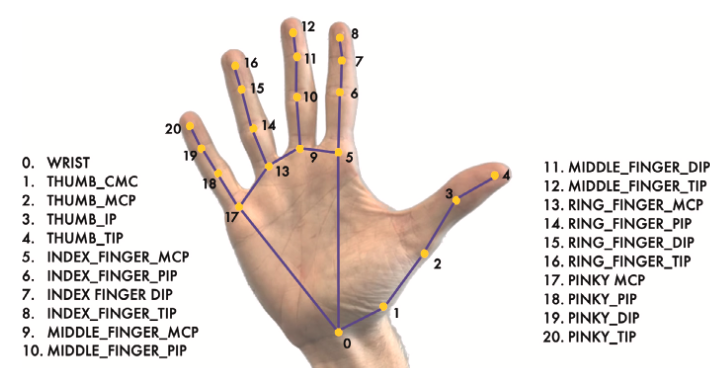
\includegraphics[width=0.5\textwidth,height=\textheight]{slike/skelet_roke.png}
\caption{COCO Hand model, tipična konfiguracija sklepov v orodjih
\emph{OpenPose} in \emph{MediaPipe}.}
\end{figure}

Torej zazanavanje drže roke oziroma položaj sklepov je večina študij
pridobila s pomočjo orodij \emph{MediaPipe}, \emph{OpenPose},
\emph{DeepLabCut} in \emph{MMPose}, ki so v zadnjih letih najbolj
uporabna. Za roko vrnejo skelet 21 točk iz katerih so potem računali
različne značilke.

\begin{figure}[H]

{\centering \includegraphics{dela_files/figure-latex/delezi orodij-1} 

}

\caption{Deleži uporabljenih orodij v preučevanih delih za sledenje rok in zaznavanje drže roke iz videoposnetkov. }\label{fig:delezi orodij}
\end{figure}

Dogajalo se je tudi, da zgornja orodja niso zaznala vseh sličic
videoposnetka in so podatki imeli mankajoče točke skeleta posameznih
sličic. Nekateri so se problema lotili z linearno interpolacijo, ki so
jo uporabili le v primeru, ko je orodje zaznalo prejšnjo in naslednjo
sličico. Posnetke, kjer orodja niso zaznala več sličic, so odstranili iz
podatkov.

Identificirali so tudi posamična gibanja tapkanja s prsti - cikel
tapkanja. Nekateri so se problema lotili z izračunom razdalje med palcem
in kazalcem oz. kotne razdalje med palcem in kazalcem in na podlagi tega
ter standardnih algoritmov določili vrh in dno amplitude oz. odpiranje
in zapiranje prstov. Večina se jih je posluževalo izračuna evklidske
razdalje med palcem in kazalcem, saj so bili koti občutljivi na nagib
kamere - med kamero in roko bi moralo biti 90 stopinj.

Orodja so v podatke vpeljela visokofrekvenčne šume, ki nastanejo zaradi
prileganja skeleta orodja roki in tremorja oseb s Parkinsonovo
boleznijo. Dobljene razdalje oz. kote so zato zgladili na različne
načine.

Nekatere študije so se lotile tudi problema neravnovesja razredov -
večina je bila uporabljen tehnika SMOTE( \emph{Synthetic Minority
Oversampling Technique}). S to tehniko so povečali manj zastopane
razrede in zmanjšali prekomerno zastopane razrede v njihovih podatkih.

Pred računanjem značilk so nekateri avtorji, predvsem tist, ki se niso
posluževali ročnega računanja značilk, podatke normalizirali z uporabo
povprečja in standardne deviacije podatkov(Z-score normalization).

\section{Značilke}\label{znaux10dilke}

Večina avtorjev je svoje modele gradila na ročno izračunanih značilkah(
\emph{manual features}) glede na smernice ocen po lestvici MDS-UPDRS.
Ker pa nekateri niso dobro poznali problema in značilnosti Parkinsonove
bolezni, ali pa so model, naučen na ročno izračunanik značilkah, želeli
primerjati, so se izračuna značilk lotili z nevronskimi mrežami. Kot
vhodni podatek so podali časovno zaporedje podatkov, model pa je iz njih
izluščil značilke.

\subsection{Ročno pridobljene
značilke}\label{roux10dno-pridobljene-znaux10dilke}

Ročno računanje značilk je temeljilo na signalih, ki so predstavljali
pospešek( \emph{acceleration}), kotna hitrost( \emph{angular velocity}),
premik( \emph{displacement}) in kot( \emph{angle}) v časovni vrsti.

Za izračun sprememb območja in hitrost tapkanja prstov so avtorji po
večini izbrali dvodimenzionalne podatke o sklepih, kjer je posamezen
sklep \(J_i\), \(i = 1, \dots, 21\)(model roke COCO) je definiran kot
\(J_i = (x_i, y_i)\) oz. tridimenzionalne podatke o sklepih, torej
posamezen sklep \(J_i\), \(i = 1, \dots, 21\)(model roke COCO) je
definiran kot \(J_i = (x_i, y_i, z_i)\), s katerimi so računali
evklidske razdalje med posameznimi sklepi v določenem časovnem okvirju,
najpogosteje razdaljo med palcem in kazalcem. Evklidska razdalja med
palcem in kazalcem v časovnem okvirju \(t\) za dvodimenzionalne podatke
je definirana kot

\[
D_t = d(J_4^t, J_8^t) = \sqrt{(x_4^t - x_8^t)^2 + (y_4^t - y_8^t)^2}
\]

oz. za trodimenzionalne podatke

\[
D_t = d(J_4^t, J_8^t) = \sqrt{(x_4^t - x_8^t)^2 + (y_4^t - y_8^t)^2 + (z_4^t - z_8^t)^2}.
\]

\begin{figure}
\centering
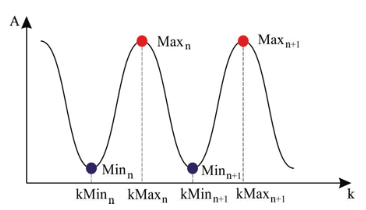
\includegraphics[width=0.5\textwidth,height=\textheight]{slike/featursi.png}
\caption{Shematična označitev odvisnosti amplitude gibanj (A) od števila
sličic (k).}
\end{figure}

\begin{itemize}
\tightlist
\item
  Število gibanj, štetih po maksimalnih točkah
\item
  Maksimalna točka med maksimalnimi točkami
\item
  Maksimalna točka med minimalnimi točkami
\item
  Minimalna točka med maksimalnimi točkami
\item
  Minimalna točka med minimalnimi točkami
\item
  Povprečno število maksimalnih točk
\item
  Standardni odklon maksimalnih točk
\item
  Povprečno število minimalnih točk
\item
  Standardni odklon minimalnih točk
\item
  število vrhov v časovnem intervalu, \(F_p\)
\end{itemize}

\subsubsection{\texorpdfstring{Amplituda( \emph{amplitude}) in hitrost(
\emph{velocity})}{Amplituda( amplitude) in hitrost( velocity)}}\label{amplituda-amplitude-in-hitrost-velocity}

Amplituda in hitrost sta dve najbolj običajni značilki, ki se
analizirata za oceno Parkinsonove bolezni z uporabo tapkanja s prsti. V
večini primerov sta definirani kot:

\emph{Amplituda: razdalja med palcem in kazalcem.}\\
\emph{Hitrost: razlika v amplitudi skozi čas.}

Iz amplitude in hitrosti so bile pogosto izračunane naslednje značilke:

\begin{itemize}
\tightlist
\item
  Povprečna, maksimalna in minimalna hitrost odpiranja in zapiranja,
\item
  povprečna, maksimalna in minimalna amplituda odpiranja in zapiranja,
  standardni odklon amplitude odpiranja in zapiranja,
\item
  povprečje in koeficient variacije amplitude gibanja,
\item
  povprečje in koeficient variacije hitrosti gibanja (amplituda gibanja
  / trajanje gibanja),
\item
  povprečje in koeficient variacije hitrosti gibanja pri odpiranju
  (amplituda gibanja / trajanje gibanja pri odpiranju),
\item
  povprečje in koeficient variacije hitrosti gibanja pri zapiranju
  (amplituda gibanja / trajanje gibanja pri zapiranju),
\item
  povprečje, koeficient variacije in razpon trajanja cikla,
\item
  hitrost gibanja (število pritiskov na čas) ter
\item
  upad amplitude (povprečna amplituda v prvi polovici poskusa v
  primerjavi s povprečno amplitudo v drugi polovici poskusa).
\item
  prelomna točka amplitude( \emph{breakpoint}), \(F_{amp- bp}\)
\item
  prelomna točka hitrosti( \emph{breakpoint}), \(F_{vel- bp}\)
\end{itemize}

\textbf{Definicija:} \emph{Amplituda odpiranja} je razlika med najvišjo
in najnižjo točko v fazi odpiranja gibanja. Izračuna se po formuli

\[
Max_n-Min_n.
\]

\textbf{Definicija:} \emph{Amplituda zapiranja} je razlika med najvišjo
in najnižjo točko v fazi zapiranja gibanja. Izračuna se po formuli

\[
Max_n-Min_{n+1}.
\]

\textbf{Definicija:} \emph{Hitrost odpiranja} je razlika med največjim
in najmanjšim vrhom v fazi odpiranja gibanja, deljena z ustreznim
časovnim intervalom. Izračuna se po formuli

\[
\frac{Max_n-Min_n}{kMax_n-kMin_n}.
\]

\textbf{Definicija:} \emph{Hitrost zapiranja} je razlika med največjim
in najmanjšim vrhom v fazi zapiranja gibanja, deljena z ustreznim
časovnim intervalom. Izračuna se po formuli

\[
\frac{Max_n-Min_{n+1}}{kMax_n-kMin_{n+1}}.
\]

\emph{Povprečje amplitude}: \[
F_{amp - mean} = \frac{\sum_{n=1}^{N}A_n}{N},
\]

kjer \(p = [p_1, p_2, \dots, p_n, \dots, p_N]\) predstavlja vrhove, kjer
je \(p_n\) \(n\)-ti vrh, \(A_n\) pa amplituda pripadajočega vrha
\(p_n\).

\emph{Varianca amplitude}: \[
F_{amp - var}\frac{\sum_{n=1}^{N}(A_n - f_{mean})^2}{N}
\]

\emph{Povprečna hitrost gibanja prsta}: \[
F_{vel - mean} = \frac{\sum_{n=1}^{N-1}V_n}{N-1},
\]

kjer je \(V_n = \frac{A_n + A_{n-1}}{\Delta t_n}\),
\(\Delta t_n = t_n - t_{n-1}\) časovni interval med \(n-1\)-tim in
\(n\)-tim vrhom amplitude.

\emph{Varianca hitrosti}: \[
F_{vel - var} = \frac{\sum_{n=1}^{N-1}(V_n - s_{mean})^2}{N-1}.
\]

\subsubsection{\texorpdfstring{Utrujenost oz. zastoj in oklevanje(
\emph{halt and
hesitation})}{Utrujenost oz. zastoj in oklevanje( halt and hesitation)}}\label{utrujenost-oz.-zastoj-in-oklevanje-halt-and-hesitation}

Utrujenost oz. zastoj in oklevanje sta lastnosti pri kateri imamo več
različnih pristopov, uporabljenih za njeno oceno. Na primer:

\begin{itemize}
\tightlist
\item
  razlika med najvišjimi in najnižjimi vrednostmi amplitudnih vrhov,
\item
  gradient amplitude glede na čas,
\item
  razlika med številom tapkanj v dveh časovnih intervalih,
\item
  koeficient variacije v hitrosti tapkanja,
\item
  razlika med povprečno vrednostjo maksimalne amplitude tapkanja prstov
  v dveh časovnih intervalih,
\item
  koeficient variacije v maksimalni amplitudi tapkanja prstov,
\item
  pospešek tapkanja.
\end{itemize}

Zastoj je bil ponavadi opredeljen kot trenutek popolne ustavitve,
oklevanje pa kot opazen upad hitrosti. Ta dva pojma so opredelili s
pomočjo vrhov \(p = [p_1, p_2, \dots, p_n, \dots, p_N]\), kjer so
uporabili model prilagajanja krivulje množici \(p\), z namenom ocene
trenda vrhov. Predpostavljamo, da je \(p_n\) vrh, ko je prišlo do
zastoja in oklevanja, \(\hat{p}_n\) pa predstavlja napovedani vrh na
podlagi prilagojenega modela. Potem je značilka zastoja in oklevanja
lahko definirana kot

\[
F_{hh} = \begin{cases}
1, \text{ če } \lvert \hat{p}_n - p_n \lvert \ge \theta \\
0, \text{ če } \lvert \hat{p}_n - p_n \lvert < \theta
\end{cases},
\]

kjer je prag( \emph{threshold}) definiran kot
\(\theta = \alpha \cdot \frac{A_{n+1}+ A_{n-1}}{2}\), \(\alpha\) je
parameter, ki nadzoruje prag, ki ga zaznamo( \emph{detection
threshold}).

\subsubsection{\texorpdfstring{Frekvenca( \emph{frequency}) oz. ritem(
\emph{rhythm})}{Frekvenca( frequency) oz. ritem( rhythm)}}\label{frekvenca-frequency-oz.-ritem-rhythm}

Uporabljata se oba pojma, ampak ne pomenita vedno isto. Izračun lahko
temelji na na uporabi hitre Fourierove transformacije( \emph{Fast
Fourier Transform}), eden izmed pristopov je tudi uporaba lastnosti
``prekrižna korelacija med normaliziranimi vrhovi''(
\emph{cross-correlation between the normalized peaks}) za oceno
doslednosti in ritma pri tapkanju.

\textbf{Definicija:} Frekvenca je enota, deljena s časovnim razponom
enega gibanja. Izračunamo jo po formuli

\[
F_{freq} = \frac{1}{kMax_{n+1} - kMax_{n}}.
\]

Računali so:

\begin{itemize}
\tightlist
\item
  povprečna frekvenca,
\item
  standardni odklon frekvence.
\end{itemize}

\subsection{Demografske značilke}\label{demografske-znaux10dilke}

Nekateri so v model vklučili tudi dva demografska dejavnika - spol in
starost. To temelji na opažanju, da naj bi lahko starejši posamezniki
kazali znake bradikinezije, povezane s staranjem, neodvisno od
Parkinsonove bolezni, ter da lahko starost in spol vplivata na razvoj
bolezni.

\subsection{Izbira značilk}\label{izbira-znaux10dilk}

Izračunane značilke so ponavadi standardizirali z uporabo metode
\emph{StandardScalar}, kar naj bi zagotvaljalo, da vse značilke enako
prispevajo k modelu in da ne bi katera izmed značilk prevadovala pri
učanju modela ali pa so bile značilke normalizirane s standardno
normalno porazdelitvijo(povprečje 0 in standardni odklon 1).

V študijah, kjer so imeli več značilk, so iskali tudi optimalno množico
značilk - značilke, ki so najpomemnejše pri klasifikaciji Parkinsonove
bolezni. Iskanje optimalne množice značilk se je razlikovalo glede na
glavo nalogo zo. cilj študije. Tisti, ki so imeli, poleg nabora podatkov
oseb s Parkinsonovo boleznijo, še nabor podatkov zdravih(kontrolnih)
oseb, so primerjali značilke, izračunane za obe skupini oseb. Značilke
so bile pregledane s pomočjo statističnega testiranja, da se ocenijo
porazdelitve v teh dveh skupinah oseb. Ker so značilke pokazale
nenormalno porazdelitev s pomočjo Shapiro-Wilkovega testa, so lahko
uporabljali Mann-Whitneyev U-test za neodvisne vzorce, za prepoznavanje
značilk, ki so v obeh skupinah oseb porazdeljene različno. Uporabljali
so značilke, ki so bile, glede na skupino oseb, porazdeljene različno.

Za izbor množice optimalnih značilk so bili uporabljeni tudi različni
algoritmi.\\
Pri algoritmu \emph{Speeded Up Robust Features}(SURF) so bile izbrane
značilke s pozitivnim rezultatom, ker to pomeni, da je značilka
stabilna, točna in potencialno uporabna za nadaljnje operacije.\\
Algritem \emph{Reursive Feature Elimination}(RFE) iterativno odstranjuje
najmanj pomembne značilke na podlagi uspešnosti modela podpornih
vekorjev(SVM), na koncu pa izbere množico, ki najbolje prispeva k nalogi
klasifikacije.\\
\emph{SelectKBest} razvršča značilke glede na njihov \emph{k-score},
metriko, ki meri relevantnost in informativnost posamezne značilke glede
na ciljno spremenljivko. Značlke, ki imajo najvišje \emph{k-score}, so
prednostno vključene v končni nabor značilk, medtem ko so manj
informativne značilke izključene.\\

Nekateri avtorji so po gradnji modelov na množici izbranih značilk
ugotovili, da izključitev določenih značilk in s tem poslabšanje
ravnovesja med značilkami povzorči poslabšanje modela, zato so se vselej
odločili za gradnjo modela na celotnem naboru značilk.

\section{Modeli}\label{modeli}

Osredotočili smo se na pregled del, kjer so izvajali klasifikacijsko
napoved, binarno ali multiklasifikacijsko. Glavni cilj študij je torej
bil implementirati model za napovedovanje ocen Parkinskonove bolezni po
letstvici MDS-UPDRS. Avtorji so za gradnjo in vrednotenje modelov
uporabljali knjižnico \emph{scikit-learn} za programski jezik Python, ki
ponuja orodja za različne naloge strojnega učenja.

\subsection{Gradnja modelov}\label{gradnja-modelov}

Večina je usposobilo en sam večrazredni klasifikacijski model, kar
pomeni, da izhod modela predstavlja vse ocene po lestvici MDS-UPDRS.
Nekateri pa so usposobili več binarnih klasifikatorjev. Nekateri
delujejo na način, da prvi model razvršča podatke videoposnetkov z oceno
0 v primerjavi z ocenami 1,2 in 3; drugi model razvršča podatke
videoposnetkov z ocenama 0 ali 1 v primerjavi z ocenami 2 ali 3; in
tretji model razvršča podatke videoposnetkov z ocenami 0, 1 ali 2 v
primerjavi z oceno 3. Uporabljen je bil tudi pristop, kjer je prvi model
razvrščal zdrave(konotrolne) osebe od oseb s Parkinsonovo boleznijo in
če je ta prvi model pokazal, da podatki videoposnetka pripadajo osebi s
Parkinsonovo boleznijo, je drugi model razvrstil ocene 1 proti ocenam 2
ali 3. In če je drugi model pokazal, oceno, višjo od 1, tretji model
razvrsti ocene 2 proti ocenam 3.

Gradili so različne modele, med najbolj pogostimi pa so bili metoda
podpornih vektorjev(SVM, \emph{Support Vector Machine}) z različnimi
jedri( \emph{karnels}), ansambli, kot sto naključni gozdovi(RF,
\emph{Random Forest}) in XBoost ter običajni klasifikatorji, kot so
odločitvena drevesa( \emph{Decision Tree}), model \(k\)-najbližjih
sosedov( \emph{\(k\)-nearest neighbors}) in logistična regresija(
\emph{logistic regression}). V zadnjih letih pa se uporabljajo tudi
globoke nevronske mreže( \emph{deep neural networks}).\\
Zaradi razlik v postopkih, podatkovnih zbirkah, nalogah klasifikacije in
uporabljenih klasifikatorjih, ne moremo podati vpogleda, kateri način
modeliranja je najboljši za klasifikacijo tapkanja s prsti po lestvici
MDS-UPDRS, so pa nekateri avtorji v prvi fazi raziskovanja zgradili več
modelov in potem, glede na rezultate, podrobno obravnavali le glavna dva
ali tri.

\begin{figure}[H]

{\centering \includegraphics{dela_files/figure-latex/delezi modelov-1} 

}

\caption{Deleži uporabljenih modelov v preučevanih delih za sledenje rok in zaznavanje drže roke iz videoposnetkov. Oznake: logistična regresija(LR), kNN(k-najbližjih sosedov), odločitvena drevesa(DT), konvolucijske nevronske mreže(CNN), metoda podpornih vektorjev(SVM), naključni gozdovi(RF).}\label{fig:delezi modelov}
\end{figure}

Pri izbiri hiperparametrov modelov so se posluževali različnih
algoritmov, kot sta RandomizeSearchCV in GridSearchCV. Pri iskanju so
uporabljali le podatke za učenje, da bi dodatno zagotovili robustnost
naučenih klasifikatorjev oz. modelov. Podatki so torej bili razdeljeni
na učne in testne, ponavadi v razmerju 70\%/30\% ali 80\%/20\%, modeli
pa usposobljeni z uporabo \(k\)-kratne navzkrižne validacije(
\emph{\(k\) - Cross Validation}), v večini primerov \(k\) = 5, nekje
celo \(k\) = 10, pri čemer so uporabljeni le podatki iz učne množice
podatkov.

\subsection{Vrednotenje modelov}\label{vrednotenje-modelov}

Za vrednotenje modelov so standardno uporabljali štiri različne metrike,
točnost( \emph{accuracy}), natančnost( \emph{precision}), priklic(
\emph{recall}) in F1, ki temeljijo tabela napačnih klasifikacij (
\emph{confusion matrix}). Pogosto je bila primerjava modelov narejena
tudi na podlagi ploščine pod krivuljo(AUC, \emph{Area Under Curve}).

\subsection{Rezultati}\label{rezultati}

V spodnjih tabelah so prikazane študije, njihovi avtorji, ter glavne
značilnosti študije - uporabljeni podatki, cilj študije, preučevan
dejavnik Parkinsonove bolezni in uporabljeni modeli strojnega učenja.

\[
\begin{table}[h]
\centering
\begin{tabular}{|l|c|r|}
\hline
Stolpec 1 & Stolpec 2 & Stolpec 3 \\ \hline
Vrstica 1 & 123       & 456       \\ \hline
Vrstica 2 & 789       & 101112    \\ \hline
\end{tabular}
\caption{Primer LaTeX tabele.}
\label{tab:tabela}
\end{table}
\]

\end{document}
